\section{Extração de Características}
\label{sec:feature-extraction}

\contentscurrent

\begin{frame}
\frametitle{Características Ideais}
\begin{itemize}
    \item Natural e frequente na fala
    \pause
    \item Facilmente mensurável
    \pause
    \item $\uparrow$ variação inter-locutor e $\downarrow$ variação intra-locutor
    \pause
    \item Constante no tempo e não afetável pela saúde
    \pause
    \item Robusto a ruído razoável e a transmissão
    \pause
    \item Difícil de ser produzido artificialmente
    \pause
    \item Não ser facilmente modificável pelo locutor
\end{itemize}
\end{frame}

\subsection{MFCC}

\begin{frame}
\frametitle{Mel-Frequency Cepstrum Coefficients}
\begin{description}
    \item Simula a função da \textbf{cóclea}
    \pause
    \item[Escala Mel] Logaritmica
    \pause
    \begin{itemize}
        \item $f_{mel} = 2595 \log_{10}(1 + \frac{f}{700})$
        \pause
    \end{itemize}
\end{description}

\begin{figure}[ht]
    \centering
    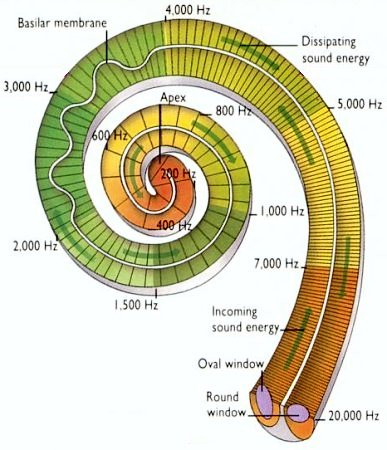
\includegraphics[width=0.35\textwidth]{cochlea}
\end{figure}
\end{frame}

\subsection{MFCC - Extração}

\begin{frame}
\frametitle{MFCC - Extração}
\begin{description}
    \item[Pré-ênfase] Realça as altas frequências (opcional)
    \pause
    \item[Janelamento] Divide o sinal em janelas superpostas
    \pause
    \item[$|FFT|^2$] Calcula o espectro de potência
    \pause
    \item[Filtros] Espectro em Hz $\implies$ espectro em mels
    \pause
    \item[dB] Calcula a sonoridade
    \pause
    \item[DCT] Coeficientes espectrais $\implies$ coeficientes cepstrais
    \pause
    \item[CMS] Normaliza os MFCCs para reduzir perturbações
    \pause
    \item[$\dvec{\Delta}$s] Novos coeficientes a partir dos antigos (opcional)
    \pause
\end{description}

\begin{figure}[ht]
    \centering
    
\includegraphics[width=0.8\textwidth]{mfcc-flow}
\end{figure}
\end{frame}